\documentclass[aspectratio=169]{beamer}
\usepackage{will_handley_beamer}
\usepackage{title_page}
\usepackage{slashed}
\usetikzlibrary{positioning}
\usetikzlibrary{calc}
\usepackage[percent]{overpic}

% Commands
% --------
% - \arxiv{arxiv number}
% - \cols{width}{lh column}{rh column}
% -  \begin{fig(left|right)}[fractional width (e.g 0.6) ]{name of image}
%        content of other column
%    \end{fig(left|right)}

% Talk details
% ------------
\title{Resonant or asymmetric: The status of sub-GeV dark matter }
\subtitle{\arxiv{2405.17548}}
\date{21\textsuperscript{st} June 2024}

\begin{document}

\begin{frame}
    \titlepage
\end{frame}

\begin{frame}
    \frametitle{Background: Dark Matter}
    \student{gambit}{}{}

    \begin{columns}
        \column{0.5\textwidth}
        \begin{itemize}
            \item We assume dark matter (DM) is a particle.
            \item If there is weak interaction with the standard model, it can be probed by  any/all of:
                \begin{itemize}
                    \item \textbf{Direct detection:} underground detector
                    \item \textbf{Indirect detection:} telescopes
                    \item \textbf{Collider searches:} missing energy
                    \item \textbf{Thermalisation:} cosmological equilibrium
                \end{itemize}
            \item Thermalisation: the same thing we search for in the lab would mean DM is in equilibrium with standard model particles at early times, but freezes out at some point.
            \item This allows us to link particles physics modelling and cosmology.
        \end{itemize}
%        \begin{tikzpicture}
%            %Diagram showing two arrows going into a circle and two arrows going out of a circle
%            \node[circle, fill=black, minimum size=3pt] (O){};
%            \node[above left = of O] (A) {};
%            \node[below left = of O] (B) {};
%            \node[above right = of O] (C) {};
%            \node[below right = of O] (D) {};
%            \draw[<->] (O) -- (A);
%            \draw[<->] (O) -- (B);
%            \draw[<->] (O) -- (C);
%            \draw[<->] (O) -- (D);
%
%            \node[rotate=-90] (X) at ($(A)!0.5!(B)$) {Normal matter};
%            \node[rotate=-90] (Y) at ($(C)!0.5!(D)$) {Dark matter};
%
%            \draw[->] (B) -- (D);
%            \draw[->] (A) -- (C);
%
%            \draw[->] (D)+(0.5,0) -- ($(C)+(0.5,0)$);
%            %\node (Z) at ($(A)!0.5!(C)$) {};
%            %\node [above = of Z] {Indirect detection};
%
%
%        \end{tikzpicture}

        
        \column{0.5\textwidth}
        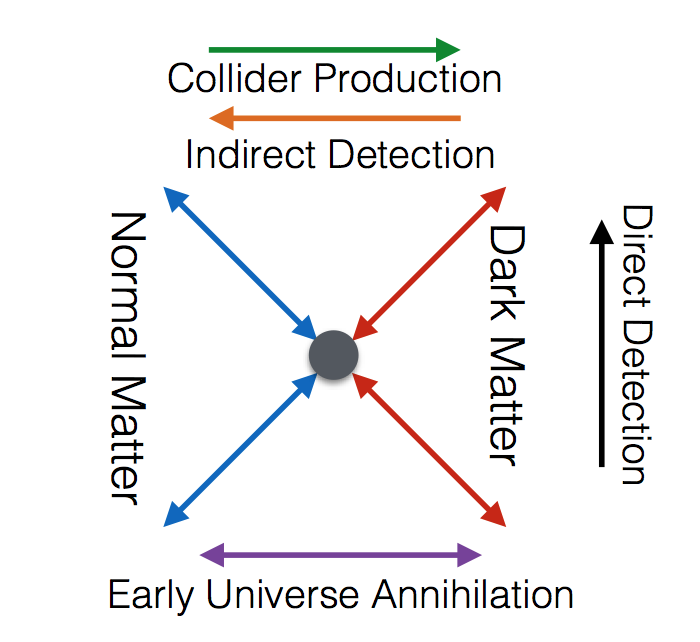
\includegraphics[width=\textwidth]{figures/DM_diagram.png}
    \end{columns}

\end{frame}

\begin{frame}
    \frametitle{Summary}
    \student{gambit}{}{}

    \begin{columns}[t]
        \column{0.48\textwidth}
        \begin{block}{Why sub-GeV?}
            \begin{itemize}
                \item If DM is a particle, $m_\text{DM}\in[10^{-30},10^{19}]~\text{GeV}$, \\\hfill($\lambda<H_0^{-1}$ and $m_\text{DM} <m_\text{p}$).
                \item If DM is thermal, $m > 10~\text{MeV}$ from CMB
                \item Direct detection means $m<1~\text{GeV}$.
                \item sub-GeV DM was thought ruled out due to Lee-Weinberg bound (known standard model interactions can't produce enough DM).
                \item However, Dark Matter + ``Dark Photons'' ($U(1)'$ gauge group) escapes this bound.
            \end{itemize}
        \end{block}
        \column{0.48\textwidth}
        \begin{block}{\arxiv{2405.17548}$=[\psi,\Phi]\times[\eta_\text{DM},\cdot]\times[f_\text{DM},\cdot]$}
            Switches we consider:
            \begin{itemize}
                \item Fermionic $\psi$ or Scalar $\Phi$
                \item symmetric $\eta_\text{DM}=0$ or asymmetric $\eta_\text{DM}\ne0$
                \item Dominant $f_\text{DM}=1$ or sub-dominant $f_\text{DM}<1$
            \end{itemize}
            We find that Fermionic, symmetric, dominant DM is disfavoured.

            The other three alternatives separately still allowed in much of the parameter space.
        \end{block}
    \end{columns}


\end{frame}

\begin{frame}
    \frametitle{Physics}
    \student{gambit}{}{}
    \begin{itemize}
        \item Dark photon $A'$ with mass $\boxed{m_{A'}}$ (via Stueckelberg mechanism) with kinetic mixing $\boxed{\kappa}$.
            \[\mathcal{L} = -\frac{1}{2}m_{A'}^2 A'_\mu A'^\mu - \frac{1}{4}A'_{\mu\nu}A'^{\mu\nu} - \kappa e A'^\mu \sum_{f\in\text{SM}} q_f \bar f \gamma_\mu f\]
        \item Dark matter candidate $\chi$ with mass $\boxed{m_\text{DM}}$, with $\chi\in\{\Phi, \psi\}$ complex scalar or Dirac fermion, coupled to the dark photon with $\boxed{g_\text{DM}}$.
        \begin{align*}
            \mathcal{L}_\psi  =& \bar{\psi}(i \slashed{\partial} - m_\text{DM}) \psi + g_\text{DM} A'^\mu \bar{\psi} \gamma_\mu \psi \\
            \mathcal{L}_\Phi  =& |\partial_\mu \Phi|^2 - m_\text{DM}^2 |\Phi|^2 - g_\text{DM}^2 A'_\mu A'^\mu |\Phi|^2 + i g_\text{DM} A'^\mu \left[\Phi^\ast (\partial_\mu \Phi) - (\partial_\mu \Phi^\ast) \Phi\right],
        \end{align*}
    \item Dark matter different from its anti-particle, there may be an asymmetry $\boxed{\eta_\text{DM}}$
    \item Also have local halo DM density $\rho_0$, velocity dispersion $v_0$ and escape velocity $v_\text{esc}$ as nuisance parameters determined by Gaia data~\arxiv{1901.02016} \textit{et al}.
    \item Focus on sub GeV region $\text{MeV} < m_\text{DM} < \text{GeV}$.
    \end{itemize}
\end{frame}

\begin{frame}
    \frametitle{Data}
    \student{gambit}{}{}
    \begin{columns}
        \column{0.49\textwidth}
        \begin{block}{Cosmological constraints}
                CMB \& BBN

            $\Omega_c h^2 \approx 0.120\pm0.001$ from \textit{Planck}

            $N_\text{eff}\approx 2.99\pm 0.17$ via \texttt{AlterBBN}
            %Exotic energy injections $p_\text{ann}$ affect recombination
        \end{block}
        \begin{block}{Astrophysical constraints}
            X-rays \& Bullet cluster

            %MeV gap (INTEGRAL $<$MeV, Fermi-LAT $>$GeV)

            %secondary signals of DM annihilation (inverse compton scattering ) producing keV X-Rays

            INTEGRAL, NuStar, XMM-Newton, Suzaku

            Bullet cluster gives self-interaction constraints%, since interactions make friction, and would cause subcluster to lose DM. (focus on the latter due to need for SBI for the former).
        \end{block}
        \column{0.49\textwidth}
        \begin{block}{Accelerator constraints}
            Beam dumps \& electron-positron colliders

            %dark photon decays into pairs of DM particles
            %constraints come from 'missing energy searches' 

            beam dump: LSND, MiniBooNE
            missing energy searches: NA64, BaBar
        \end{block}
        \begin{block}{Direct detection constraints}
            searches for electron \& nuclear recoils

            Xenon1T, SENSEI, DarkSide50, PandaX-4T, DAMIC-M, SuperCDMS HV
        \end{block}
    \end{columns}
\end{frame}

{
    \usebackgroundtemplate{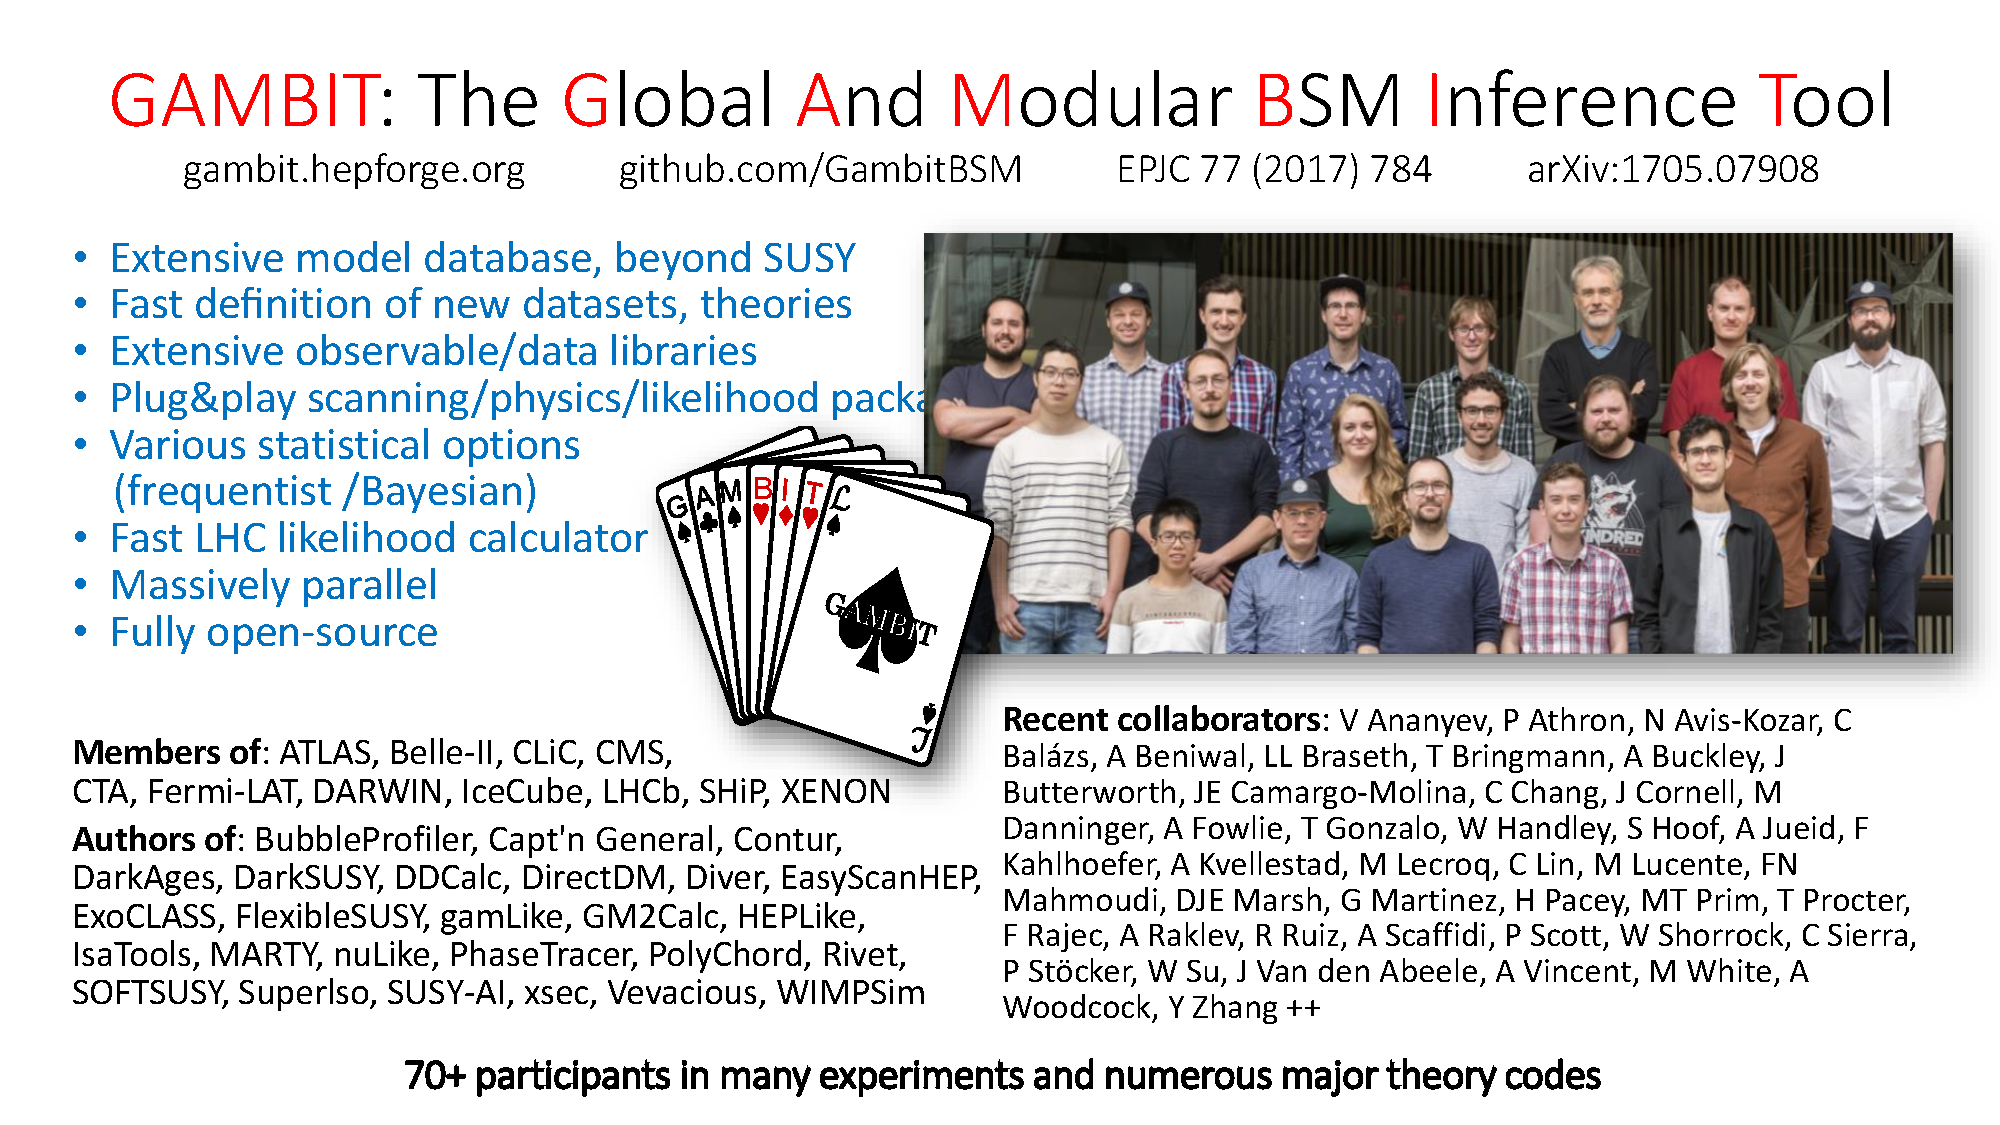
\includegraphics[width=\paperwidth]{gambit_ad_slide}}
    \begin{frame}[plain]
    \end{frame}
}

%\begin{frame}
%    \frametitle{GAMBIT: combining datasets}
%    \begin{columns}
%        \column{0.5\textwidth}
%        \begin{itemize}
%            \item GAMBIT is an interdisciplinary community and software framework.
%            \item Like \texttt{CosmoMC}/\texttt{Cobaya}/\texttt{Bilby}, an organiser of data, likelihoods \& theory, including:
%                \begin{itemize}
%                    \item Collider data (e.g. LHC)
%                    \item Direct detections (e.g. XENON1T)
%                    \item Cosmology (\texttt{MontePython})
%                    \item Astrophysics (e.g. Bullet Cluster, Supernovae)
%                    \item Pulsar timing
%                    \item \ldots \& much more
%                \end{itemize}
%            \item \texttt{GravBit} and \texttt{LowEnergyBit} arising from GAMBIT@KICC workshop
%        \end{itemize}
%        \column{0.5\textwidth}
%        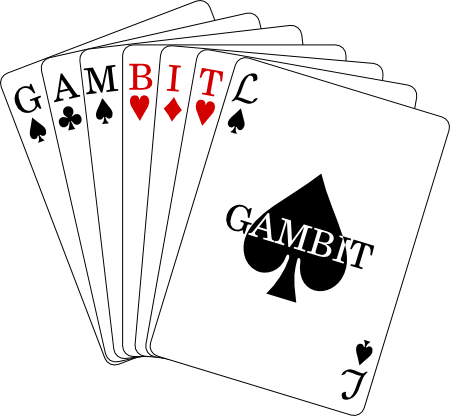
\includegraphics[height=0.423\textwidth]{figures/students/gambit.png}
%        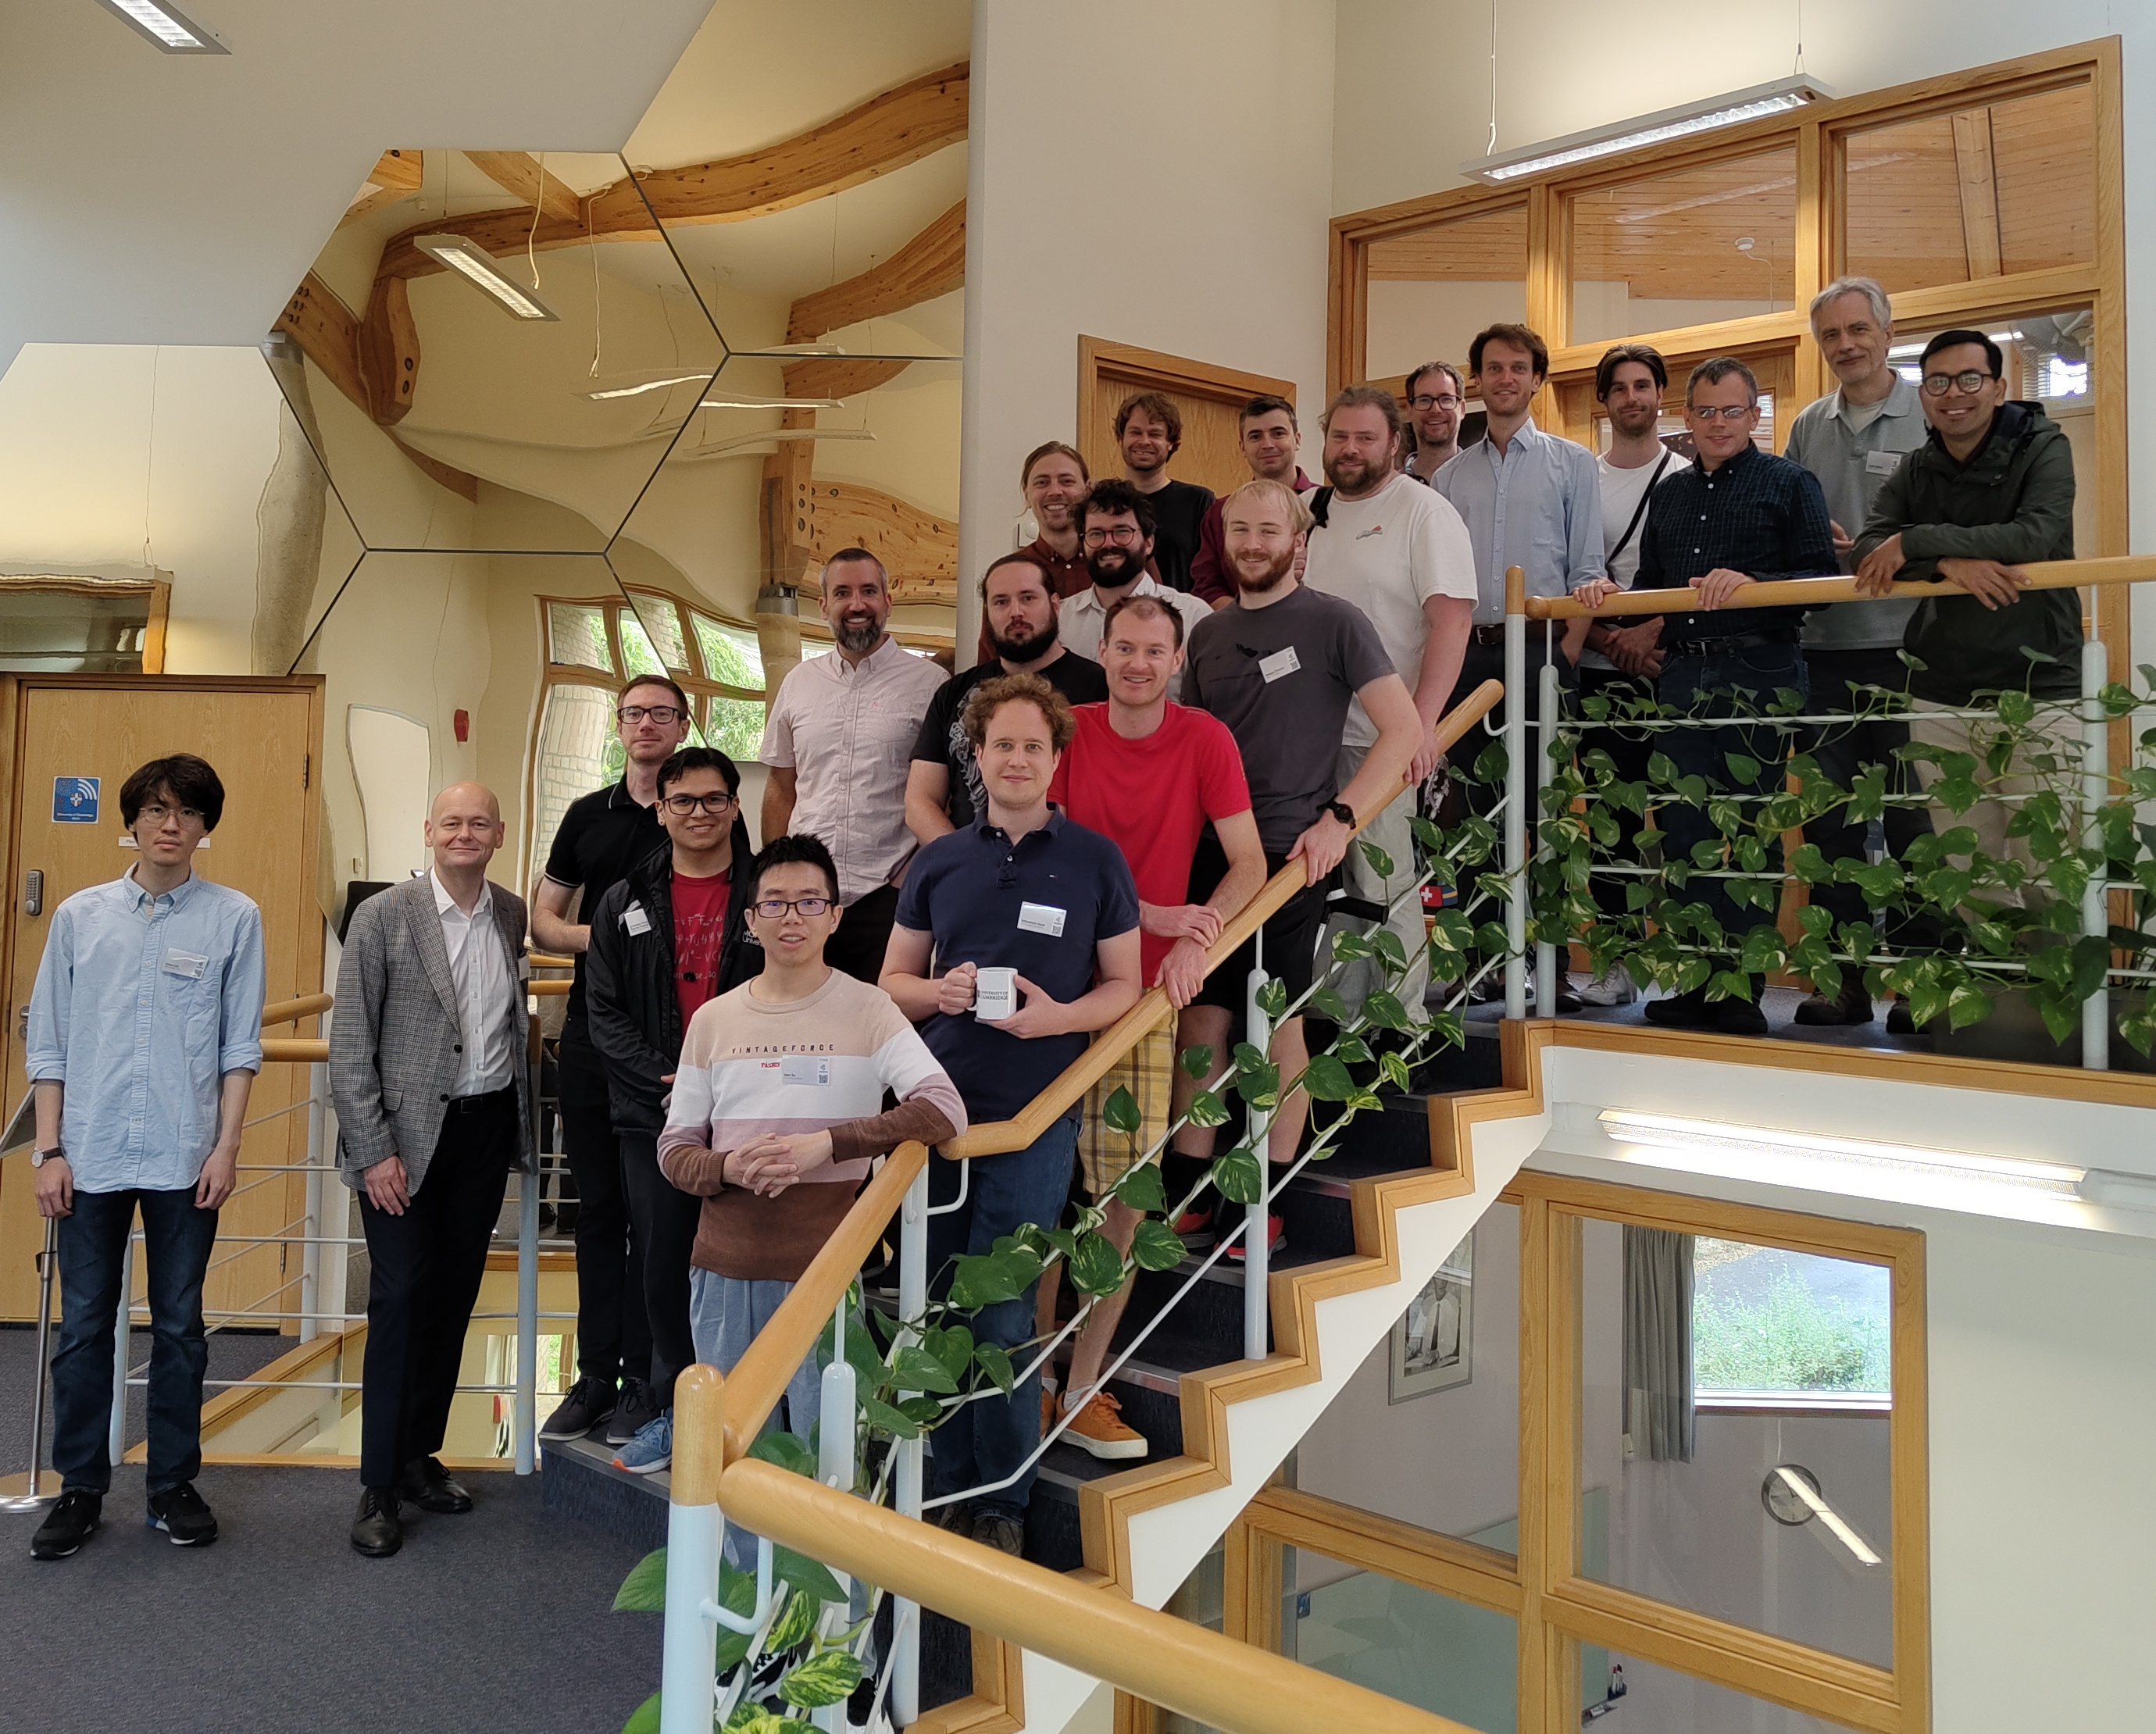
\includegraphics[height=0.423\textwidth]{figures/gambit_kicc.jpg}
%        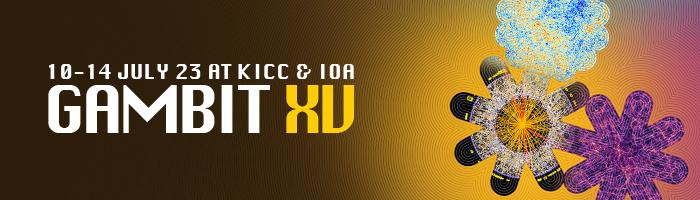
\includegraphics[width=\textwidth]{figures/gambit_meetingbanner.jpg}
%    \end{columns}
%\end{frame}


%\begin{frame}
%    \frametitle{What is GAMBIT?}
%    \student{gambit}{}{}
%    \vspace{-10pt}
%    \begin{columns}
%        \column{0.48\textwidth}
%        \begin{block}{GAMBIT as a software framework}
%            \begin{itemize}
%                \item Combines collider, direct detection, neutrino \& telescope data.
%                \item Allows joint analysis of dark matter, neutrinos \& BSM physics
%                \item MPI + OpenMP parallelisation \\(record of 115,000 CPUs)
%                \item Combines libraries \& codes written in:\\
%                    \texttt{C++}, \texttt{Fortran}, \texttt{Python}, \texttt{Mathematica}\ldots
%                \item Highly modular ``Bits''
%                \item Often with several alternatives
%            \end{itemize}
%        \end{block}
%        \column{0.48\textwidth}
%        \begin{block}<only@1>{GAMBIT as a community}
%            \begin{itemize}
%                \item Particle physicists, cosmologists \& statisticians ($>$80 members)
%                \item Generates interdisciplinary expertise \& inspires new techniques
%                \item Open source software
%                \item Access to large community computing resources (40MCPUh/y)
%                \item Modularity allows parallel teams
%                \item Short-author papers by default
%                \item in-person meetings every 9 months
%            \end{itemize}
%        \end{block}%
%        \includegraphics<2>[width=\textwidth]{figures/gambit_kicc.jpg}
%    \end{columns}
%\end{frame}


\begin{frame}
    \frametitle{Parameter estimation}
    \student{gambit}{}{}
    \begin{columns}
        \column{0.4\textwidth}
        \begin{itemize}
            \item Frequentist analysis: Profile likelihood plots optimise unseen parameters 
            \item Can build intuition for how data constrain parameters
            \item Global fit extracts more information than traditional particle physics approach
            %    \begin{itemize}
            %        \item Useful for ``worst case''/guarantee statements
            %    \end{itemize}
            %\item Bayesian analysis: Posterior probability plots marginalise  unseen parameters
            \item Grey contours have $f_\text{DM}\le1$.
            \item Similar plots for fermions.
            \item Asymmetric dark matter less constrained.
            \item GAMBIT can do Bayesian \& Frequentist analyses.
        \end{itemize}
        
        \column{0.6\textwidth}
        \only<1>{
            \begin{overpic}[width=\textwidth]{figures/fermion_mDM_epsR.pdf} 
            \put(45,70) {\small Indirect detection}
            \put(55,65) {\small $\epsilon_R\lesssim 0.4$}
            \end{overpic}
        }%
        \includegraphics<2>[width=\textwidth]{figures/fermion_mDM_gDM.pdf}%
        \only<3>{
            \begin{overpic}[width=\textwidth]{figures/fermion_mDM_kappa.pdf} 
            \put(45,25) {\tiny Relic density requirements}
            \end{overpic}
        }%
        \only<4>{
            \begin{overpic}[width=\textwidth]{figures/fermion_gDM_kappa.pdf} 
            \put(45,35) {\tiny Relic density requirements}
            \end{overpic}
        }
        \only<5>{
            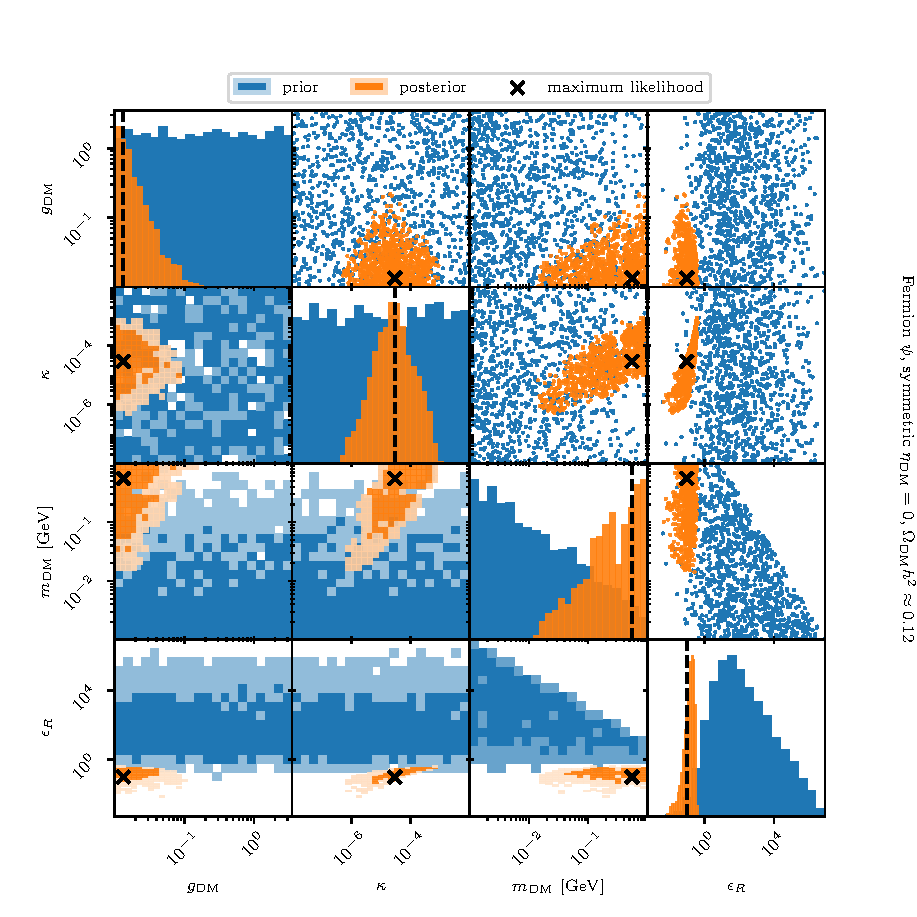
\includegraphics[width=0.79\textwidth]{figures/Bayes_SubGeVDM_fermion_allDM_sym.pdf}
        }
    \end{columns}
\end{frame}


\begin{frame}
    \frametitle{Model comparison}
    \student{gambit}{}{}
    \includegraphics<1>[width=\textwidth]{figures/allDM.pdf}
    \begin{columns}
        \column{0.5\textwidth}
        \begin{itemize}
            \item Fermionic symmetric dark matter disfavoured
                \includegraphics<2->[width=\textwidth]{figures/allDM.pdf}
            \item<2-> This is because the the cross sections with SM need to be more fine-tuned.
            \item<2-> contrasts with scalar as it's easier to generate dark matter without asymmetry ($p$-wave suppression of annihilation cross section).
        \end{itemize}
        \column{0.5\textwidth}
        \vspace{0.6em}
        \includegraphics<2>[width=\textwidth]{figures/Bayes_SubGeVDM_fermion_allDM_sym_observables.pdf}%
        \includegraphics<3>[width=\textwidth]{figures/Bayes_SubGeVDM_fermion_RDprior_allDM_asym_observables.pdf}
    \end{columns}
\end{frame}

\begin{frame}
    \frametitle{Conclusions}
    \student{gambit}{}{}
    \framesubtitle{\tthref{gambitbsm.org}}
    \begin{columns}
        \column{0.5\textwidth}
            \begin{itemize}
                \item GAMBIT \texttt{DarkBit}, \texttt{CosmoBit} \& \texttt{ScannerBit} modules now mature enough to fit principled dark matter models to a wide variety of data.
                \item Unique combination of tools \& expertise that can systematically test dark matter models.
                \item Future detectors will constrain these further.
                \item Looking for other possible contributions to GAMBIT physics-driven global fits
            \end{itemize}
        \column{0.5\textwidth}
        \includegraphics<1>[width=\textwidth]{figures/fermion_asym_mAp_kappa_sensitivities.pdf}%
        \includegraphics<2>[width=\textwidth]{figures/fermion_asym_mDM_fsigmap_sensitivities.pdf}%
        \includegraphics<3>[width=\textwidth]{figures/fermion_asym_mDM_fsigmae_sensitivities.pdf}
    \end{columns}
\end{frame}

\end{document}
